\documentclass[../../main.tex]{subfiles}
\begin{document}

{\bf [解答]}

与えられた条件
\begin{align}
  \begin{cases}
    -\dfrac{\pi}{2} \le \alpha, \beta \le \dfrac{\pi}{2} \\
    \sin(x+\alpha) + \sin(x+\beta) = \sqrt{3}\sin x
  \end{cases} \label{eq:1}
\end{align}
について考える．題意より\cref{eq:1}の第二式が$x$ についての恒等式なので，
$x = 0, \dfrac{\pi}{2}$ での成立が必要で
\begin{align}
  \begin{cases}
    \sin\alpha + \sin\beta = 0 \\
    \cos\alpha + \cos\beta = \sqrt{3}
  \end{cases} \label{eq:2}
\end{align}
である．\cref{eq:1}の第一式と\cref{eq:2}の第一式から
\begin{align}
  \beta = -\alpha \label{eq:3}
\end{align}
である．

\begin{figure}[htb]
  \centering
  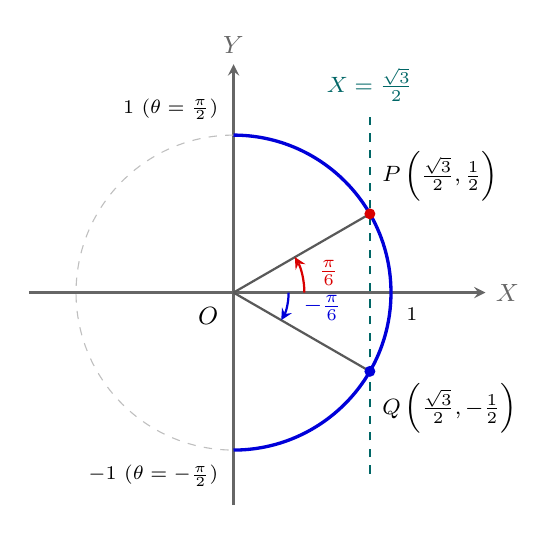
\begin{tikzpicture}[scale=2.0, >=stealth,
    every node/.style={font=\small}]
    \coordinate (O) at (0, 0);

    % 座標軸
    \draw[->, thick, gray!80!black] (-1.3, 0) -- (1.6, 0) node[right] {$X$};
    \draw[->, thick, gray!80!black] (0, -1.35) -- (0, 1.45) node[above] {$Y$};
    \node[below left=2pt] at (O) {$O$};

    % 単位円（定義域外の左半分は薄い破線、定義域内の右半分は実線強調）
    \draw[dashed, gray!50] (0, 1) arc (90:270:1);
    \draw[line width=1.2pt, blue!85!black] (0, -1) arc (-90:90:1);

    % 直線 X = \sqrt{3}/2
    \pgfmathsetmacro{\xval}{sqrt(3)/2}
    \pgfmathsetmacro{\yval}{0.5}
    \draw[line width=0.9pt, teal!80!black, dashed] (\xval, -1.15) -- (\xval, 1.15)
    node[above, font=\footnotesize, teal!80!black] {$X = \frac{\sqrt{3}}{2}$};

    % 動径 OP, OQ
    \coordinate (P) at (\xval, \yval);
    \coordinate (Q) at (\xval, -\yval);
    \draw[line width=0.8pt, gray!70!black] (O) -- (P);
    \draw[line width=0.8pt, gray!70!black] (O) -- (Q);

    % 角の弧
    \draw[->, thick, red!85!black] (0.45, 0) arc (0:30:0.45);
    \node[right=1pt, red!85!black, font=\footnotesize] at (15:0.48) {$\frac{\pi}{6}$};
    \draw[->, thick, blue!85!black] (0.35, 0) arc (0:-30:0.35);
    \node[right=1pt, blue!85!black, font=\footnotesize] at (-15:0.38) {$-\frac{\pi}{6}$};

    % 円周上の点
    \node[circle, fill=red!85!black, inner sep=1.4pt] at (P) {};
    \node[above right=1pt, font=\footnotesize] at (P) {$P\left(\frac{\sqrt{3}}{2}, \frac{1}{2}\right)$};
    \node[circle, fill=blue!85!black, inner sep=1.4pt] at (Q) {};
    \node[below right=1pt, font=\footnotesize] at (Q) {$Q\left(\frac{\sqrt{3}}{2}, -\frac{1}{2}\right)$};

    % 目盛り・端点ラベル
    \node[below right=2pt, font=\scriptsize] at (1, 0) {$1$};
    \node[above left=2pt, font=\scriptsize] at (0, 1) {$1 \ (\theta = \frac{\pi}{2})$};
    \node[below left=2pt, font=\scriptsize] at (0, -1) {$-1 \ (\theta = -\frac{\pi}{2})$};
  \end{tikzpicture}
  \caption{単位円上における角 $\alpha, \beta$ の決定}
  \label{fig:unit_circle_angles}
\end{figure}

\cref{eq:2}の第二式に代入して
\begin{align}
  2\cos\alpha = \sqrt{3}
  \iff
  \cos\alpha = \dfrac{\sqrt{3}}{2}
  \iff
  \alpha = \pm\dfrac{\pi}{6} \quad (\because\text{\cref{eq:1}})
\end{align}
を得る．\cref{eq:3}と合わせて
\begin{align}
  (\alpha, \beta) = \left( \pm\dfrac{\pi}{6}, \mp\dfrac{\pi}{6} \right) \quad (\text{複号同順})
\end{align}
が必要である．逆にこの時，\cref{eq:1}の左辺は
\begin{align}
  (\text{左辺}) = 2\sin x \cos\dfrac{\pi}{6} = \sqrt{3}\sin x = (\text{右辺})
\end{align}
となって十分である．よって求める$\alpha,\beta$は
\begin{align}
  (\alpha, \beta) = \left( \pm\dfrac{\pi}{6}, \mp\dfrac{\pi}{6} \right) \quad (\text{複号同順})
\end{align}
である．

\end{document}
